%preamble - package inclusion and set up
\documentclass[12pt,twoside,a4paper,english]{report}

% Select encoding of your inputs
\usepackage[utf8]{inputenc}

% Make latex understand and use the typographic
% rules of the language used in the document.
%\usepackage[danish]{babel}
\usepackage[english]{babel}

% Use the vector font Latin Modern which is going
% to be the default font in latex in the future.
\usepackage{lmodern}

% Choose the font encoding
\usepackage[T1]{fontenc}

% Use color in tables
\usepackage[table]{xcolor}
\usepackage{pbox}
\usepackage{tabularx}
\usepackage{array}
\usepackage{multirow}

% Load a colour package
\usepackage{xcolor}
\definecolor{aaublue}{RGB}{33,26,82}  %<--define aaublue
\definecolor{white}{RGB}{255,255,255} %<--define white

% ref stuffz
\usepackage{cleveref}

% The standard graphics inclusion package
\usepackage{graphicx}

\makeatletter
  \g@addto@macro\@floatboxreset\centering %<--centering all figures
\makeatother

\usepackage{adjustbox}

% Set up how figure and table captions are displayed
\usepackage{float}
\usepackage{caption}
\usepackage{subcaption}
\captionsetup
{
  justification = centering,    %<--centering caption with multiple lines
  font          = footnotesize, %<--set font size to footnotesize
  labelfont     = bf            %<--bold label (e.g., Figure 3.2) font
}
\captionsetup[subfigure]
{
  justification = centering, %<--centering subfigure caption text
  singlelinecheck=false,
  font = footnotesize        %<--font size for subfigures
} 

% Enable row combination in tables
\usepackage{multirow}

% Make space between table lines and text
\renewcommand{\arraystretch}{1.5}

% Enable commands like \st (strike out) and \hl (high light)
\usepackage{soul}

% Make the standard latex tables look so much better
\usepackage{array,booktabs}

% Enable the use of frames around, e.g., theorems
% The framed package is used in the example environment
\usepackage{framed}
\usepackage{colortbl}
\usepackage{longtable}
\usepackage{xcolor}
\usepackage{textcomp}

%-------MATHEMATICS---------------------------------
% Defines new environments such as equation,
% align and split 
\usepackage{amsmath}
\usepackage{relsize}
% Adds new math symbols
\usepackage{amssymb}
% Use theorems in your document
% The ntheorem package is also used for the example environment
% When using thmmarks, amsmath must be an option as well. Otherwise \eqref doesn't work anymore.
\usepackage[framed,amsmath,thmmarks]{ntheorem}
\usepackage{xifthen}%<--enables ifthenelse which is used in macros

\usepackage{siunitx} 
\sisetup{decimalsymbol=period}%<--\num{} will swich commas with periods
\sisetup{detect-weight}
%---------------------------------------------------

%-------PAGE LAYOUT---------------------------------
% Change margins, papersize, etc of the document
\usepackage[
  left=25mm,% left margin on an odd page %tidligere 25mm for baade right og left
  right=25mm,% right margin on an odd page
  top=35mm,
  ]{geometry}
  
% Modify how \chapter, \section, etc. look
% The titlesec package is very configureable
\usepackage{titlesec}
\makeatletter
\def\ttl@mkchap@i#1#2#3#4#5#6#7{%
    \ttl@assign\@tempskipa#3\relax\beforetitleunit
    \vspace{\@tempskipa}%<<<<<< REMOVE THE * AFTER \vspace
    \global\@afterindenttrue
    \ifcase#5 \global\@afterindentfalse\fi
    \ttl@assign\@tempskipb#4\relax\aftertitleunit
    \ttl@topmode{\@tempskipb}{%
        \ttl@select{#6}{#1}{#2}{#7}}%
    \ttl@finmarks  % Outside the box!
    \@ifundefined{ttlp@#6}{}{\ttlp@write{#6}}}
\makeatother

\titlespacing{\chapter}{0pt}{0pt}{10pt}
\titlespacing{\section}{0pt}{0pt}{-5pt}
\titlespacing{\subsection}{0pt}{8pt}{-5pt}
\titlespacing{\subsubsection}{0pt}{6pt}{-10pt}

\titleformat*{\section}{\normalfont\Large\bfseries\color{aaublue}}
\titleformat*{\subsection}{\normalfont\large\bfseries\color{aaublue}}
\titleformat*{\subsubsection}{\normalfont\normalsize\bfseries\color{aaublue}}

\usepackage{titlesec, blindtext, color}
%\color{gray75}{gray}{0.75}
\newcommand{\hsp}{\hspace{20pt}}
\titleformat{\chapter}[hang]{\Huge\bfseries}{\thechapter\hsp\textcolor{aaublue}{|}\hsp}{0pt}{\Huge\bfseries}

% Change the headers and footers
\usepackage{fancyhdr}
\setlength{\headheight}{15pt}
\pagestyle{fancy}
\fancyhf{} %delete everything
\renewcommand{\headrulewidth}{0pt} %remove the horizontal line in the header
\fancyhead[RO,LE]{\color{aaublue}\small\nouppercase\leftmark} %even page - chapter title
\fancyhead[LO]{}
\fancyhead[RE]{} 
\fancyhead[CE]{}
\fancyhead[CO]{}
\fancyfoot[RE,LO]{\thepage}
\fancyfoot[LE,RO]{} %page number on all pages
\fancyfoot[CE,CO]{}

% change first page of all chapters header and footer to fancy style
\makeatletter
\let\ps@plain\ps@fancy
\makeatother

% Do not stretch the content of a page. Instead,
% insert white space at the bottom of the page
\raggedbottom

% Enable arithmetics with length. Useful when typesetting the layout.
\usepackage{calc}
%---------------------------------------------------

\usepackage{appendix}

%-------BIBLIOGRAPHY--------------------------------
%setting references (using numbers) and supporting i.a. Chicargo-style:
\usepackage{etex}
\usepackage{etoolbox}
\usepackage{keyval}
\usepackage{ifthen}
\usepackage{url}
\usepackage{csquotes}
\usepackage[backend=biber, url=true, doi=true, style=numeric, sorting=none]{biblatex}
\addbibresource{setup/bibliography.bib}
%---------------------------------------------------

%-------MISC----------------------------------------
%%% Enables the use FiXme refferences. Syntax: \fxnote{...} %%%
\usepackage[footnote, draft, english, silent, nomargin]{fixme}		%!!!! DRAFT OR FINAL?!?!?!?!11!! change later!	
%With "final" instead of "draft" an error will ocure for every FiXme under compilation.

%%% allows use of lorem ipsum (generate i.e. pagagraph 1 to 5 with \lipsum[1-5]) %%%
\usepackage{lipsum}

%%% Enables figures with text wrapped tightly around it %%%
\usepackage{wrapfig}

%%% Section debth included in table of contents (1 = down to sections) %%%
\setcounter{tocdepth}{1}

%%% Section debth for numbers (1 = down to sections) %%%
\setcounter{secnumdepth}{2}

\usepackage{tocloft}
\setlength{\cftbeforetoctitleskip}{0 cm}
\renewcommand{\cftpartpresnum}{Part~}
\let\cftoldpartfont\cftpartfont
\renewcommand{\cftpartfont}{\cftoldpartfont\cftpartpresnum}
%---------------------------------------------------

%-------DANSK SPROG---------------------------------

%\addto\captionsdanish{%
%	\renewcommand{\figurename}{figur}%
%	\let\figureautorefname\figurename%
%	\renewcommand{\tablename}{tabel}%
%	\let\tableautorefname\tablename%
%%	\renewcommand{\equationname}{ligning}%
%%	\let\equationautorefname\equationname%
%	\renewcommand{\chaptername}{Kapitel}%
%	\let\chapterautorefname\chaptername%
%	\renewcommand{\partname}{Del}%
%	\let\partautorefname\partname%
%	\renewcommand{\sectionname}{afsnit}%
%	\let\sectionautorefname\sectionname%
%%	\renewcommand{\thesubsection}{underafsnit}%
%%	\let\subsectionautorefname\thesubsection%
%	\renewcommand{\pagename}{side}%
%	\let\pageautorefname\pagename%
%}

%-------HYPERLINKS----------------------------------
% Enable hyperlinks and insert info into the pdf
% file. Hypperref should be loaded as one of the 
% last packages
\usepackage{nameref}
\usepackage{hyperref}
\usepackage{bookmark}
\hypersetup{%
	%pdfpagelabels=true,%
	plainpages=false,%
	pdfauthor={Author(s)},%
	pdftitle={Title},%
	pdfsubject={Subject},%
	bookmarksnumbered=true,%
	colorlinks,%
	citecolor=aaublue,%
	filecolor=aaublue,%
	linkcolor=aaublue,% you should probably change this to black before printing
	urlcolor=aaublue,%
	pdfstartview=FitH%
}

\crefname{appsec}{bilag}{bilag}
%---------------------------------------------------

% remove all indentations
\setlength\parindent{0pt}
\parskip 5mm
\usepackage{verbatim}

\definecolor{Gra}{RGB}{230,230,230}

%creates a nice-looking C#-text
\newcommand{\CC}{C\nolinebreak\hspace{-.05em}\raisebox{.3ex}{\scriptsize\text \#} }

%enables multi column lists
\usepackage{multicol}

%enables code-examples
\usepackage{listings}

\definecolor{coolblue}{RGB}{32,95,128}
\definecolor{mygreen}{rgb}{0,0.6,0}
\definecolor{mygray}{rgb}{0.5,0.5,0.5}
\definecolor{mymauve}{rgb}{0.58,0,0.82}
\usepackage{textcomp}
\definecolor{listinggray}{gray}{0.9}
\definecolor{lbcolor}{rgb}{0.9,0.9,0.9}

%for c code
\lstdefinestyle{cstyle}{
  backgroundcolor=\color{lbcolor},
	tabsize=4,
	rulecolor=,
	language=C,
  basicstyle=\scriptsize,
  upquote=true,
  aboveskip={1.5\baselineskip},
  columns=fixed,
  showstringspaces=false,
  extendedchars=true,
  breaklines=true,
  prebreak = \raisebox{0ex}[0ex][0ex]{\ensuremath{\hookleftarrow}},
  frame=single,
  showtabs=false,
  numbers=left,
  captionpos=b,
  numbersep=5pt,
  numberstyle=\tiny\color{mygray},
  showspaces=false,
  showstringspaces=false,
  identifierstyle=\ttfamily,
  keywordstyle=\color[rgb]{0,0,1},
  commentstyle=\color[rgb]{0.133,0.545,0.133},
  stringstyle=\color[rgb]{0.627,0.126,0.941},
}
%for python code
\lstdefinestyle{pythonstyle}{
    backgroundcolor=\color{lbcolor},
    tabsize=4,
    rulecolor=,
    language=python,
    basicstyle=\scriptsize,
    upquote=true,
    aboveskip={1.5\baselineskip},
    columns=fixed,
    showstringspaces=false,
    extendedchars=true,
    breaklines=true,
    prebreak = \raisebox{0ex}[0ex][0ex]{\ensuremath{\hookleftarrow}},
    frame=single,
    showtabs=false,
    numbers=left,
    captionpos=b,
    numbersep=5pt,
    numberstyle=\tiny\color{mygray},
    showspaces=false,
    showstringspaces=false,
    identifierstyle=\ttfamily,
    keywordstyle=\color[rgb]{0,0,1},
    commentstyle=\color[rgb]{0.133,0.545,0.133},
    stringstyle=\color[rgb]{0.627,0.126,0.941},
}
%for matlab code
\lstdefinestyle{matlabstyle}{
    backgroundcolor=\color{lbcolor},
    tabsize=4,
    rulecolor=,
    language=Matlab,
    basicstyle=\scriptsize,
    upquote=true,
    aboveskip={1.5\baselineskip},
    columns=fixed,
    showstringspaces=false,
    extendedchars=true,
    breaklines=true,
    prebreak = \raisebox{0ex}[0ex][0ex]{\ensuremath{\hookleftarrow}},
    frame=single,
    showtabs=false,
    numbers=left,
    captionpos=b,
    numbersep=5pt,
    numberstyle=\tiny\color{mygray},
    showspaces=false,
    showstringspaces=false,
    identifierstyle=\ttfamily,
    keywordstyle=\color[rgb]{0,0,1},
    commentstyle=\color[rgb]{0.133,0.545,0.133},
    stringstyle=\color[rgb]{0.627,0.126,0.941},   
}

%for java code
\lstdefinestyle{javastyle}{
	backgroundcolor=\color{lbcolor},
	tabsize=4,
	rulecolor=,
	language=Java,
	basicstyle=\scriptsize,
	upquote=true,
	aboveskip={1.5\baselineskip},
	columns=fixed,
	showstringspaces=false,
	extendedchars=true,
	breaklines=true,
	prebreak = \raisebox{0ex}[0ex][0ex]{\ensuremath{\hookleftarrow}},
	frame=single,
	showtabs=false,
	numbers=left,
	captionpos=b,
	numbersep=5pt,
	numberstyle=\tiny\color{mygray},
	showspaces=false,
	showstringspaces=false,
	identifierstyle=\ttfamily,
	keywordstyle=\color[rgb]{0,0,1},
	commentstyle=\color[rgb]{0.133,0.545,0.133},
	stringstyle=\color[rgb]{0.627,0.126,0.941},
}

%for inline c, syntax: \cline{ codeHere(); }
\lstdefinestyle{cinline}{
    style=cstyle,
    basicstyle=\small,
}
\newcommand\inlinec[1]{ \lstinline[style=cinline]{#1} }

%for inline python, syntax: \pythonline{ codeHere(); }
\lstdefinestyle{pythoninline}{
    style=pythonstyle,
    basicstyle=\small,
}
\newcommand\inlinepython[1]{ \lstinline[style=pythoninline]{#1} }

%for inline matlab, syntax: \matlabline{ codeHere(); }
\lstdefinestyle{matlabinline}{
    style=matlabstyle,
    basicstyle=\small,
}
\newcommand\inlinematlab[1]{ \lstinline[style=matlabinline]{#1} }

\usepackage{enumitem}
%\usepackage[citestyle=authoryear,natbib=true]{biblatex}

% Figures - TIKZ
\usepackage{tikz}
\usepackage[americanresistors,americaninductors,americancurrents, americanvoltages]{circuitikz}

% Wall of text logo
\newcommand{\walloftextalert}[0]{\includegraphics[width=\textwidth]{walloftext.png}}

\usepackage{pdfpages}
\usepackage{lastpage}
\usepackage{epstopdf}

\setlength{\headheight}{21pt}

\hfuzz=\maxdimen
\tolerance = 10000
\hbadness  = 10000

\usepackage{siunitx}
\graphicspath{{./figures/}}

%macros - please read this file
%Macro for 'where'-enviroment was improved by Andrea and Niels :-)

%-----------UNITS-------------------------------------------
\newcommand{\unit}[1]{&& \left[\si{#1}\right]}
%
%\newcommand{\unit}[1]{[\si{#1}]}            %<<| Use these if you want equations to be
%\newcommand{\eq}[2]{&&\si{#1} &= \si{#2}&&} %<<| centered.. .. will appear scrambled
%                                            %  | from one equation to the next though..
%                                            %  | and does not work with long equations.. :/
%
%-----------------------------------------------------------

%-----------WHERE ENVIRONMENT-------------------------------
\newenvironment{where}{\leavevmode{\parindent=1em\indent} Where:\\}{}
\newcommand{\va}[3]
{
  \begin{tabular}{p{20pt} p{40pt} p{290pt} l}
    & { $#1$ } & { #2 } & \ifthenelse{\isempty{ #3 }}  {}  {[{\si{#3}}]} \\
  \end{tabular}\\
}
%-----------------------------------------------------------

%-----------TikZ SETTINGS-----------------------------------
\tikzset{
  block/.style    = {draw, thick, rectangle,
                     minimum height = 2.1em,
                     minimum width = 1.7em},
  sum/.style      = {draw, circle, inner sep=3pt} %<--Adder
}
%-----------------------------------------------------------


%-----------Fanzy reference SETTINGS------------------------
%Figure references:
\newcommand{\figref}[1]{figure \ref{#1}}

%Figure references after full stop/period:
\newcommand{\Figref}[1]{Figure \ref{#1}}

%Table references:
\newcommand{\tabref}[1]{table \ref{#1}}

%Table references after full stop/period:
\newcommand{\Tabref}[1]{Table \ref{#1}}

%Section references:
\newcommand{\secref}[1]{section \ref{#1} on site \pageref{#1}}

%Section references:
\newcommand{\Secref}[1]{Section \ref{#1} on site \pageref{#1}}

%Appendix references:
\newcommand{\appref}[1]{appendix \ref{#1} on site \pageref{#1}}

%Appendix references:
\newcommand{\Appref}[1]{Appendix \ref{#1} on site \pageref{#1}}

%chapter references: 
\newcommand{\chapref}[1]{chapter \ref{#1} on site \pageref{#1}}

%chapter references: 
\newcommand{\Chapref}[1]{Chapter \ref{#1} on site \pageref{#1}}

%Units:
%\newcommand{\unit}[1]{&& \left[\si{#1}\right]}

%Text:
\newcommand{\tx}[1]{\text{#1}}

%Equation references:
%1 equation:
\renewcommand{\eqref}[1]{equation (\ref{#1})}

%-----------------------------------------------------------





\begin{document}       % TIP: If you are using TeXstudio you can open
%\tableofcontents      %      the file by Ctrl+LeftClick on setup/macros.tex
\pagebreak             %      If the file doesn't exist, you will be asked
					   %      weather or not you want to create it.


%||||||||||||||||||||||||||||||||||||||||||||||||||||||||||||||||
%|||||||                 Example Inputs                  ||||||||
%||||||||||||||||||||||||||||||||||||||||||||||||||||||||||||||||
%|||||||                                                 ||||||||
%			 \chapter{Figure Sample}

\begin{figure}[H]                                         %   File-type can be specified
  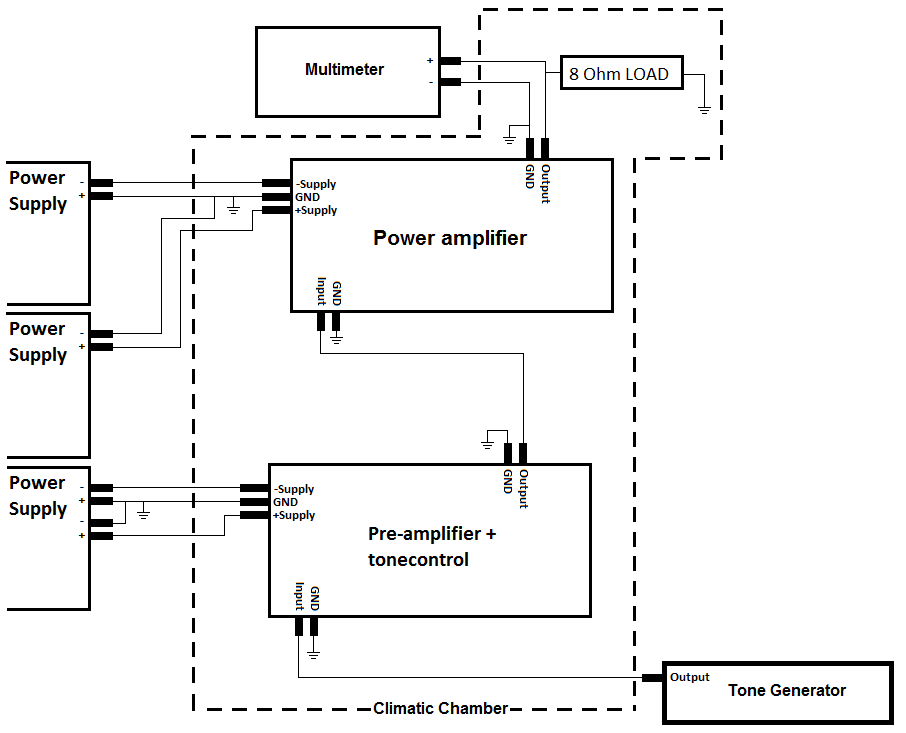
\includegraphics[width=.4\textwidth]{figures/filename}  %<--but is not needed.
  \caption{This image is clearly too small, remember to scale appropriately \fxnote{Remember source}}
  \label{fig:FigureLABEL}  %<--give the figure a label, so you can reference!
\end{figure}               %   For the label to work it must be under the caption.

% Fxnotes will not compile properly inside the figure, only in the caption.
% When \fxnote{} is used in caption, it does not show in a footnote as it normally 
% would, it does however appear in list of corrections.

\autoref{fig:FigureLABEL} $\leftarrow$ use autoref, unless you are referring to multiple pictures, then do like this: \autoref{fig:HbridgeClokwise4Q} and \ref{fig:HbridgeCounterClokwise4Q}.

%Do NOT use \vspace{length}, \hspace{length} or \noindent etc. unless exceedingly necessary - LaTeX is a markup language, let it do its job.
\vspace{.5cm}
\noindent
%
%--------- BIBLIOGRAPHY REF EKSAMPLE -----------------------------------
This reference only represents this line since it is before the punctuation mark\cite{YDing}. This next reference however represents the entire section. That is, all of the preceding sentences in the entire section. This is due to the fact that it is now after the punctuation mark in the end of the section (this is not used in the middle of a section!).\cite{YDing}

%>>PLEASE ALSO READ THE NOTE IN bibliography/bibliography.bib<<

Here is a way to make two images appear on the side of each other. Also, if you modified an image, this is how you properly refer to its original source:

\begin{figure}[H]
    \subcaptionbox  %<--use captionbox instead if no global caption is needed
    {               %                                \%-%-%-%-%-%-%\
      Clockwise 4Q operation.\newline                              %\
      \emph{Edited from image by Biezl.\cite{Biezl}}                %\
      \label{fig:HbridgeClokwise4Q}                                  %\
    }                                                                 %\
    {                                                                  %\
      \includegraphics[width=.46\textwidth]{HbridgeClockwise4Q}         %\
    }                                                                    %\
    \hspace{5pt}                                                          %\
    \subcaptionbox  %<-----------------------------------------------------%\
    {                                                                       %\
      Counterclockwise 4Q operation.\newline                                 %\
      \emph{Edited from image by Biezl.\cite{Biezl}}                          %\
      \label{fig:HbridgeCounterClokwise4Q}                                     %\
    }                                                                           %\
    {                                                                            %\
      \includegraphics[width=.46\textwidth]{HbridgeCounterClockwise4Q}            %|
    }                                                                             %|
    \caption{The 4 quadrant H-bridge configuration shown in both directions.}%<-%-/
    \label{fig:Hbridges}
\end{figure}

As seen \autoref{fig:HbridgeCounterClokwise4Q} can be referred to on its own, or you can use \autoref{fig:Hbridges} to refer to both \autoref{fig:HbridgeClokwise4Q} and \autoref{fig:HbridgeCounterClokwise4Q}.

If the figures are not directly related you might not want to use \textbf{(a)} and \textbf{(b)}, but instead give each figure their own label, here is an example:

\begin{figure}[H]
    \captionbox
    {
      Clockwise 4Q operation.\newline
      \emph{Edited from image by Biezl.\cite{Biezl}}
      \label{fig:HbridgeClokwise4Q2}
    }
    {
      \includegraphics[width=.46\textwidth]{HbridgeClockwise4Q}
    }
    \hspace{5pt}
    \captionbox
    {
      Counterclockwise 4Q operation.\newline
      \emph{Edited from image by Biezl.\cite{Biezl}}
      \label{fig:HbridgeCounterClokwise4Q2}
    }
    {
      \includegraphics[width=.46\textwidth]{HbridgeCounterClockwise4Q}
    }
\end{figure}

In this case \autoref{fig:HbridgeClokwise4Q2} can be referred to without involving \autoref{fig:HbridgeCounterClokwise4Q2}.

\pagebreak			 %|||||||
%			 \section{Table Sample} %to view this sample properly in the code, the screen must be
                       %wide enough, or you have to disable word-wrap in your editor.
\begin{table}[H]
\begin{tabular}{|l|p{5cm}|l|l|l|}
  \hline %-----------------------------------------------------------------------------------
  \textbf{No.} &\textbf{Description} &\textbf{Min} &\textbf{Max} &\textbf{Requirements}    \\
  \hline %-----------------------------------------------------------------------------------
  1            & Some Text           & Some Text   & Some Text   & Some Text               \\
               &                     &             &             & Some More Text          \\
               &                     &             &             & Text Text               \\
               &                     &             &             & Text Text Text          \\
  \hline %-----------------------------------------------------------------------------------
  2            & Some Text           & Some Text   & Some Text   & Some Text               \\
  \hline %-----------------------------------------------------------------------------------
  3            & By specifying the
                 width of a column
                 (|p\{5cm\}|) the
                 cells in that column
                 will not exceed the
                 specified width but         %Extra whitespace is used only for clarity
                 instead expand              %and will not affect the compiled output.
                 downward.
                                     & Some Text           & Some Text   & Some Text       \\
  \hline %-----------------------------------------------------------------------------------
  4            & Some Text           & Some Text   & Some Text   & Some Text               \\
  \hline %-----------------------------------------------------------------------------------
  \multicolumn{2}{|l|}{Some Text}    & \multicolumn{3}{l|}{Some Text}                      \\
  \hline %-----------------------------------------------------------------------------------
  \multicolumn{2}{|l|}{Text Text}    & \multicolumn{3}{l|}{Text = Text}                    \\
  \multicolumn{2}{|l|}{}             & \multicolumn{3}{l|}{Text = Text}                    \\
  \multicolumn{2}{|l|}{}             & \multicolumn{3}{l|}{Text = Text}                    \\
  \multicolumn{2}{|l|}{}             & \multicolumn{3}{l|}{Text = Text}                    \\
  \multicolumn{2}{|l|}{}             & \multicolumn{3}{l|}{Text = Text}                    \\
  \hline %-----------------------------------------------------------------------------------
  \multicolumn{2}{|l|}{Some Text}    & \multicolumn{3}{l|}{Teeeexxtt}                      \\
  \multicolumn{2}{|l|}{}             & \multicolumn{3}{l|}{\LaTeX}                         \\
  \hline %-----------------------------------------------------------------------------------
\end{tabular}
\caption{This Is a Table\label{table:TableLABEL}}
\end{table}

\autoref{table:TableLABEL} $\leftarrow$ use autoref, unless you are referring to multiple tables, then do like this: \autoref{table:TableLABEL} and \ref{table:TableLABEL}.

\pagebreak 		     %|||||||
%			 \section{Equation Sample} %<--In American English all Important Words in
                          %   Headlines are with Big Letters

% \unit is a macro. It uses SI units and aligns all the units neatly :)

\textbf{A normal equation:}
\begin{flalign}
  J_m \cdot \dot{\omega}_m(t) &= \tau_m(t) - B_m \cdot \omega_m(t) - r_m \cdot f_c(t)& \unit{N \cdot m}
  \label{eq:MotorGearNewtonSecLaw}
\end{flalign}
%
\begin{where}
  \va{ J_m               }{is the motor's inertia}                     {kg \cdot m^2}
  \va{ \omega_m(t)       }{is the angular velocity of the motor}       {rad \cdot s^{-1}}
  \va{ \dot{\omega}_m(t) }{is the angular acceleration of the motor}   {rad \cdot s^{-2}}
  \va{ \tau_m(t)         }{is the torque delivered by the motor}       {N \cdot m}
  \va{ B_m               }{is the motor's friction coefficient}        {N \cdot m \cdot s \cdot rad^{-1}}
  \va{ r_m               }{is the radius of the gear, $G_m$}           {m}
  \va{ f_c(t)            }{is the contact force between the two gears} {N}
\end{where}

\textbf{If you need to write something with numbers:} %<--Do not use \textbf{} as headlines, it is bad practice
                                                      %   use instead \chapter{}, \section{}, \subcaption{}, \subsubsection{}
                                                      %   in that order - never a \subsubsection{} directly under a \section{}
\begin{flalign}
  B      &= \num{2,2}\cdot 10^{-6}  \ \si{N\cdot m \cdot rad^{-1} \cdot s}& \label{eq:eq2} \\ %<-- if you want two equations to
  \tau_c &= \num{0.0016}            \ \si{N\cdot m}                       & \label{eq:eq3}    %    allign in one envirenment,
\end{flalign}                                                                              %    remember \\
%using \num{} ensures the same use of decimal point throughout the repport
%should you want to change it, the option is set in the preamble, just change 'period' to 'comma':
%\sisetup{decimalsymbol=period}

\autoref{eq:MotorGearNewtonSecLaw} $\leftarrow$ use autoref, unless you are referring to multiple equations, then do like this: \autoref{eq:eq2} and \ref{eq:eq3}.

\pagebreak		 %|||||||
%			 \section{TikZ Sample}

\textbf{TikZ is only for very patient people, I can recommend Inkscape with textext plugin: \url{https://pav.iki.fi/software/textext/}, difficult to install easy to use, and, if used carefully, nice results.}

%heavily commented example
\input{chapters/tikz/TikZblockDiagramSample.tex}

%way to keep the drawing code in a seperate file
\begin{figure}[H]
	\input{chapters/tikz/smallBlockDiagram.tikz}
	\centering
	\caption{Block diagram}
\end{figure}

%TikZ can also be used for circuits
\input{chapters/tikz/TikZcircuitSample.tex}


\pagebreak            %|||||||
%			 \section{Code Sample}

\begin{lstlisting}[ style=cstyle,
                    caption={C Code}, 
                    label=lst:cExample ]
#include "functions.h"

// Constant matrices
const float L[3] = { -11.0, -12.0, -13.0 };
const float B1[4] = { 0.0, -0.2396, 0.0, 0.2396 };
const float B2[4] = { 0.2396, 0.0, -0.2396, 0.0 };
const float B3[4] = { 0.0377, -0.0377, 0.0377, -0.0377 };
\end{lstlisting}

In \autoref{lst:cExample} is some C-code, and here is some in-line C-code: \inlinec{xTaskCreate();}.

\begin{lstlisting}[ style=pythonstyle,
                    caption={Python Code}, 
                    label=lst:pythonExample ]
# This parses the packets to identify messages and decodes them for the logs
class packetParser():
    def __init__(self,accelfile,gpsfile,measstate,fulllog,plog):
        self.GPS = {0: 'Latitude',
                    1: 'Longtitude',
                    2: 'Velocity'}
        self.IMU = {0: 'AccelerationX',
                    1: 'AccelerationY',
                    2: 'AccelerationZ',
                    3: 'GyroscopeX',
                    4: 'GyroscopeY',
                    5: 'GyroscopeZ',
                    6: 'MagnetometerX',
                    7: 'MagnetometerY',
                    8: 'MagnetometerZ',
                    9: 'Temperature'}
        self.MsgID = {0: self.GPS, 1: self.IMU}
        self.DevID = {0: 'GPS', 1: 'IMU'}
        self.accelburst = [0,0,0,0,0,0,0]
        self.accellog = accelfile
        self.fulllog = fulllog
\end{lstlisting}

In \autoref{lst:pythonExample} is some Python-code, and here is some in-line Python-code:\\ \inlinepython{self.plog.write(str(msgnr))}

\begin{lstlisting}[ style=matlabstyle,
                    caption={Matlab Code}, 
                    label=lst:matlabExample ]
  close all
  clear
  clc
  
  % Parameters
  mx=200;     % [kg] mass + added mass in xb direction
  my=250;     % [kg] mass + added mass in yb direction
  Iz=700;     % [kgm2]
  
  dx=70;      % [kg/s] 
  dy=100;     % [kg/s]
  dyaw=50;    % [kgm2/s]
\end{lstlisting}

In \autoref{lst:cExample}, \ref{lst:pythonExample} and \ref{lst:matlabExample} is some code, and here is some in-line matlab: \inlinematlab{randn(50)}            %|||||||
%|||||||                                                 ||||||||
%||||||||||||||||||||||||||||||||||||||||||||||||||||||||||||||||
%||||||||||||||||||||||||||||||||||||||||||||||||||||||||||||||||


%%% Prereport %%%
\setlength\cftaftertoctitleskip{2pt}
\setlength\cftafterloftitleskip{6pt}
\setlength\cftafterlottitleskip{6pt}
%\selectlanguage{danish}
\title{Ingen ved det}

%%% Frontmatter Settings %%%
\pagestyle{empty} %disable headers and footers
\pagenumbering{roman} %use roman page numbering in the frontmatter I II...
\fancyfoot[RE,LO]{17gr6407} %page number on all pages
\fancyfoot[LE,RO]{\thepage}
\fancyhead[LE,LO,RE,RO]{}

%%% Introductory Formalities %%%
%\includepdf[pages={1}]{formalities/frontpage.pdf}
%\clearpage
\thispagestyle{empty}

\begin{figure}[H]
	\raggedleft
	
\includegraphics[width=0.2\textwidth]{figures/aaulogo-da.png}
\end{figure} 

\vspace{5 cm}

\begin{center}	
	\begin{Huge}
		\textbf{System til facilitering af motivation hos KOL-patienter}\\
		\vspace{5 mm}
		P$6$ Bachelorprojekt - Foråret $2017$\\
		\vspace{3 mm}
	\end{Huge}
	{\Large Gruppe $17$gr$6407$}
\end{center}
\vspace*{\fill}

\begin{center}
	\line(1,0){400}
\end{center}


\pagestyle{fancy}
%{\small
\strut\vfill % push the content to the bottom of the page
\noindent Copyright \copyright{} Aalborg University 2015\par
\vspace{0.2cm}

\noindent This report is compiled in \LaTeX, originally developed by Leslie Lamport, based on Donald Knuth's \TeX. The main text is written in \emph{Latin Modern} pt 12, designed by Bogusław Jackowski and Janusz M. Nowacki. 
%The document is compiled via the website \url{www.overleaf.com}, an online collaborative based \LaTeX-editor with instant preview, which enables multiple persons to edit the document simultaneously.
Flowcharts and diagrams are made using Microsoft Visio. 
\clearpage
%%\begin{document} 
\thispagestyle{empty}
\begin{titlepage}
\begin{nopagebreak}
{\samepage 

\begin{tabular}{r}
\parbox{\textwidth}{  \raisebox{-15mm}{
\includegraphics[height=3cm]{figures/aaulogo-da.png}}
\hfill \hspace{2cm} \parbox{8cm}{\begin{tabular}{l} %4.90
{\small \textbf{\textcolor{aaublue}{{1\textsuperscript{st} Semester, Project}}}}\\
{\small \textbf{\textcolor{aaublue}{School of Medicine and Health}}}\\
%{\small \textbf{\textcolor{aaublue}{Communication Technologies}}}\\ 
{\small \textbf{\textcolor{aaublue}{Biomedical Engineering and Informatics}}}\\
{\small \textcolor{aaublue}{Fredrik Bajers Vej 7A}} \\
{\small \textcolor{aaublue}{9220 Aalborg}} \\
%{\small \textcolor{aaublue}{\emph{http://www.sict.aau.dk/electronics-and-it}}}
\end{tabular}}}
\end{tabular}

\begin{tabular}{cc}
\parbox{7cm}{

\textbf{Title:}

Thermal imaging as method to study the effect of induced ischemia on vasomotion \\ 

\textbf{Theme:}

\small{
 Biomedical Signals and Informatics\\
}


\parbox{8cm}{


\textbf{Project period:}\\
P1, Fall 2017\\
01/09/2017 - 20/12/2017\\
   
\textbf{Projektgruppe:}\\
17gr7407\\ %\fxnote{Input group number}
  
\textbf{Participants:}\\
Annabel Bantle \\
Christian Korfitz Mortensen\\
Toby Steven Waterstone\\



\textbf{Supervisors:}\\
Lasse Østergaard\\
Carsten Dahl Mørch\\
Andrei Ciubotariu
}\\
\\
\\
\textbf{Pages:} 52\\
\textbf{Appendix:} 6 \\
%\textbf{Ekstra:} For projektkode: Se forord\\ %eks. en CD eller USB
\textbf{Handed in:} 20/12/2017\\
\\
\textit{The content of this report is freely available, but publication (with reference) may only be done with
	agreement with the author.}
\vfill } &
\parbox{7cm}{
  \vspace{.15cm}
  \hfill
  \begin{tabular}{l}
  {\textbf{Synopsis}}\bigskip \\
  \fbox{
    \parbox{6.5cm}{\bigskip
     {\vfill{\small Vasomotion is an autoregulatory mechanism that optimizes blood distribution within the microcirculatory system. Thermal imaging is a promising approach to measure this phenomena.	
Previous studies have detected that vasomotion is quantifiable as temperature micro oscillations in the endothelial (0.005 - 0.02 Hz), neurogenic (0.02 - 0.05 Hz) and myogenic (0.05 - 0.15 Hz) frequency band. Four healthy subjects were recruited to investigate the possibilities of measuring changes in vasomotric activity caused by partial occlusion of blood supply by using thermal imaging.
Measurements were done as a baseline and with 50\% restriction of hand$’$s blood supply by brachial cuff.
No significant difference between the mean magnitudes of baseline and restriction was found. 
Results showed thermal imaging might not be sensitive enough to detect vasomotion and clear limitations in the experimental setup.
     \bigskip}}
     }}
   \end{tabular}}
\end{tabular}} %\vspace{1cm}


%\centering
%\textit{Offentliggørelse af rapportens indhold, med kildeangivelse, må kun ske efter aftale med forfatterne.}\\

\end{nopagebreak}
\end{titlepage}
%\end{document}
%%% Preface %%%
%\cleardoublepage
%\chapter*{Abstract}
Chronic obstructive pulmonary disease (COPD) is among the leading causes of death worldwide and patients suffering from the disease slowly deteriorate as it progresses. Studies have shown that physical exercise is beneficial to patients suffering from COPD, however some patients are unable or unwilling to leave their homes in order to exercise. This project aims to answer the question of how to motivate COPD patients to exercise and thus improving their general state of health. As an answer to this question a system has been developed which can motivate COPD patients to exercise from home, while still allowing healthcare personnel to monitor their activity. The system is developed mainly using object-oriented programming and the development process is described using unified modeling language. The system is split into three main components; a hardwaremodule for measuring the crankarms revolutions on an exercise bike, a front-end application that displays distance and other information about the training session, and a back-end system with a database and a user interface for healthcare personnel to monitor the patients activiy. 
\clearpage
%\chapter*{Preface}

Needs to be written 

-Tell about us as group, the place we study, something about the study \\
-Thank the supervisors 

\pagebreak

\pdfbookmark[0]{Table of Contents}{label: tableOfCentents}
\tableofcontents
\cleardoublepage


%%% Mainmatter Settings %%%
\pagenumbering{arabic} %use arabic page numbering in the mainmatter
\fancyfoot[RO,LE]{\thepage \text{ of} \pageref{LastPage}}
\fancyfoot[RE,LO]{17gr6407}
\fancyhead[RE,LO]{}
\fancyhead[RE,LO]{\color{aaublue}\small\nouppercase\leftmark} %even page - chapter title
\pagestyle{fancy}


%---------------------------INPUTS-------------------------------

\part{Background}
%Physiology
\chapter{Anatomy and Physiology}
\textit{The following chapter will outline the functions of the cardiovascular system and focuses on its microcirculatory part. Further the phenomena of vasomotion will be explained.}


\section{Macrocirculatory system}
The main function of the cardiovascular system is the blood supply of the whole body and the transportation of metabolites. The propulsion of this is the heart. It generates the systolic blood pressure through the strength of left ventricle. The pressure difference between the heart and the periphery emerging from there, ensures the blood flow. The blood flows from regions with high pressure, like the aorta, to regions with low pressure, like the periphery.\cite{martini2012}

The heart supplies the body through the systemic and the pulmonary circuit with blood. Through these circuits the heart regulates the blood allocation with adjustment of stroke volume and heart frequency. The oxygen-rich blood accumulates in the left ventricle. From there the blood is pushed out through the aortic valve into the aorta and via the arteries spread into the whole body. The venous system returns the meanwhile low in oxygen blood back to the heart into the right atrium. From there the blood flows into the right ventricle and is pushed out through the pulmonary valve into the lung arteries. In the lungs gas exchange of the blood happens. Subsequent the oxygen-rich blood flows via the pulmonary veins back to the left heart to supply the body.\cite{martini2012}

As mentioned, there are two types of vessels, arteries and veins. The difference between those two types of vessels is that arteries transport the blood away from the heart and veins solely transport blood to the heart. There are also some differences in the structure of arteries and veins.
Arteries consist of three different layers, tunica interna, tunica media and tunica externa. The tunica interna consists of vascular endothelium, the tunica media consists of smooth muscle cells and elastic fibres, the tunica externa consists of connective tissue and also elastic fibres. Furthermore, there are two different types of arterial vessels. In arteries of the elastic type prevail the elastic fibres in the tunica media. This allows an abrupt extension of the vessel during the systole and ensuing constriction, due to this the blood is transported. This phenomena is called windkessel function. In arteries of the muscular type prevail the muscular fibres in the tunica media. This allows regulation of the lumen by constriction and dilatation, whereby the resistance and the blood flow in the organs is regulated.\cite{martini2012}

Venous vessels are similarly structured like arterial vessels, however they are thinner and have also semilunar valves inside, to inhibit back flow inside the vessels. This system is supported by the skeletal muscles which help to hold up blood flow. The arterial and the venous vessel system are connected through the capillary system in the microcirculatory system.\cite{martini2012}


\section{Microcirculatory system}

The heart and larger arteries and veins are associated with the cardiovascular system, but those are only used for transportation of blood. Instead it is the capillaries, that permeate most tissues, that is responsible for the perfusion of tissue. These are the only vessels which permit exchange between the vessel and the surrounding interstitial fluids.  Factors that affect tissue perfusion is cardiac output, peripheral resistance and blood pressure. Capillaries are made not of single individual fluid conductors like veins and arteries, but instead formed into capillary beds. Here they work as a interconnected network of vessels.
As mentioned before the arteries decrease in size the further they expand into the peripheral system. The small arteries divide into arterioles which further divide into dozen of capillaries. The capillaries merge into a venule after the blood has been de-oxygenated. A capillary is divided into two segments, first the metarteriole and second the capillary. The blood flow between arterioles and venules can also be a direct connection, made by an arteriovenous anastomosis. This works as a bypass diverting blood flow around the capillary bed. An example of the structure of the capillary bed can be seen on \cref{fig:beds}.\cite{martini2012}
\begin{figure}[H]                                         
	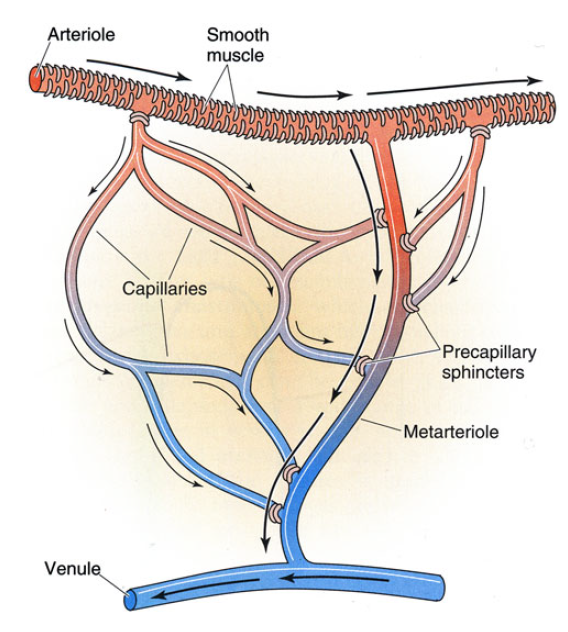
\includegraphics[width=.6\textwidth]{figures/capillary_bed}  
	\caption{The basic structure of a capillary bed, with arteriole on the left side of the bed and a venule on the right\cite{martini2012}.}
	\label{fig:beds}  
\end{figure}          

Each capillary entrance is controlled by a precapillary sphincter, which is composed of smooth muscle cells, that are able to contract or relax and thereby limit access of blood flow to certain capillaries. The blood flows relatively slow within the capillaries giving time for the two way exchange of nutrients and wastes. \cite{martini2012}

\subsection{Vasomotion}

The flow within the capillaries varies. This is among other thing due to the earlier mentioned precapillary sphincters opening and closing. The opening and closing of sphincters is part of the autoregulation process performed at a local level, to control the blood flow. The vascular system does not contain blood enough for every vessel a capillary beds to be filled with blood. Therefore only $25\%$ of the vessels in a capillary bed contains blood, and vessels activity needs to be well coordinated. Thermoregulation and control of nutrition balance are the primary functions of the microcirculatory system. Local changes in concentration of chemicals and interstitial fluids eg. dissolved oxygen concentrations in tissue modulates the vascular smooth muscles activity. Constriction and dilation of the vessel is thereby regulated by this periodic activity, also known as vasomotion. \cite{martini2012,geyer2004}

Under normal circumstances cardiac output remains stable and the control of local blood flow happens through local peripheral resistance within local tissues. The regulation of cardiovascular activity is controlled by local homeostatic mechanism. These make sure that demands such as oxygen and nutrients are meet and wastes are disposed.\cite{martini2012}

Physiological mechanism controlling vasomotion are not yet fully understood, but vascular smooth muscle activity has been shown to be roughly proportional to the tissue’s metabolic demand for oxygen.\cite{geyer2004}
Further have some factors that trigger homeostatic mechanism to alter the vasomotion been said to have an impact. Factors that trigger dilation is called vasodilators and can be some of the following:\cite{martini2012,geyer2004}  
\begin{itemize}
	\item Decreased oxygen level or increased CO2 level
	\item Lactic acid or other acids generated from tissue cells
	\item Nitric oxide NO released from endothelial cells
	\item Rising concentrations of potassium ions or hydrogen ions in the interstitial fluid
	\item Chemicals released during local inflammation
	\item Elevated local temperature
\end{itemize} 

A vasodialation will result in increased oxygen, nitrients, buffers released to recreate homeostasis.
Factors that stimulate contriction is called vasoconstricters and can happen due to following:\cite{martini2012} 

\begin{itemize}
	\item Damaged tissue
	\item Aggregating platelets 
\end{itemize}





%Hemodynamics
\chapter{Hemodynamics}
Hemodynamics explains the movement or flow of blood. It is influenced by parameters like blood pressure, blood volume, cardiac output, blood composition, etc. It is possible to measure some of the hemodynamic parameters non-invasive, and also to calculate parameters.\cite{martini2012,thiriet2008}

\section{Physiological Base}
The regulation of the blood pressure happens with baroreceptors in the walls of the big arteries in chest and neck area. These receptors register the changes of the elongation of the vessels and transmit this information to medulla oblongata. With the received pressure informations  initiates the medulla oblongata, if necessary, regulatory measures. For the short-term regulation is the sympathicus responsible. Both, middle-term and long-term regulation, is made by the kidneys. For middle-term regulation messenger substance are released, which entail vasoconstriction. The long-term regulation occurs  per pressure diuresis or reabsorption in the kidneys.It is possible to measure different blood pressures at different places in the cardiovascular system, for example the mean arterial pressure $(MAP)$. The $ MAP $ increases in relation to the stroke volume and decreases when blood flows into the peripheral system.\cite{martini2012,thiriet2008} \\

The cardiac output $ (CO) $ states the blood volume, which is pumped by the heart per time unit $(HR)$. The calculation of the $ CO $ as follows.\cite{martini2012}
\begin{flalign}
	CO=HR\times stroke volume
\end{flalign}


\section{Physical Base}
To consider the hemodynamics, it is possible to draw conclusions by analogy of physical laws. Especially of Ohm's law $ R=\frac{U}{I} $ or rather $ I=\frac{U}{R} $. A special case of Ohm's law constitutes Hagen-Poiseuille's law in the field of fluid dynamic and rheology. Hagen-Poiseuille's law describes the laminar flow of an homogeneous Newtonian fluid through a rigid pipe depending on characteristics of the fluid and of the pipe.\cite{noordergraaf2011,thiriet2008}

Blood is an inhomogeneous suspension of liquid and corpuscular components, whose viscosity $ \eta $ depends on more factors than the temperature, and is consequently no Newtonian fluid. Nevertheless it is possible to draw conclusions by analogy out of Hagen-Poiseuille's law for the computation of the hemodynamics.\cite{noordergraaf2011,thiriet2008}
\begin{flalign}
	\frac{V}{t}=\frac{r^{4}\times\pi\times\Delta P}{8\times\eta\times I}
\end{flalign}

Here is the volume flow equivalent to the electrical current $ I $ and the pressure difference $ \Delta $P to the electric voltage $ U $. Thus, the calculation of the resistance as follows.\cite{noordergraaf2011,thiriet2008}
\begin{flalign}
	R=\frac{8\times I\times\eta}{r^{4}}
\end{flalign}

Thereby volume flow increases 16 times and the resistance decreases 16 times for double radius $ r $.\cite{noordergraaf2011,thiriet2008}\\

%Pathalogy 
\chapter{Pathology}
This chapter describes pathologic incidents in the cardiovascular system and organs during sepsis.

\label{chap:sepsis}
\section{Sepsis and Vasomotion}

Sepsis is a condition, which develops through systemic inflammatory response syndrome (SIRS) with presence of an infection or bacteria within the body. Sepsis adversely affect heart rate, blood pressure, oxygen extraction and body temperature and leads to multi organ failure in worst cases.\cite{pluta2010,kanta2014}

Since sepsis is based on an inflammation, the body activates the inflammatory cascade as an immune response. Some factors released by the inflammatory cascade have influence on vasodilation and triggers a dispersed systemic vasodilation and decrease the responsiveness of the affected vasculature. It is known that sepsis leads to imbalance of the microcirculation, whereby the blood distribution becomes unequal. Areas with a lack of blood supply which already have a need of blood might get less blood, whereas areas with sufficient supply might get more of the available amount of blood. As an adequate oxygen supply requires a sufficient circulation, the condition of the areas with a lack of blood supply deteriorates.
If local microcirculation of several organs like kidneys or liver is impaired over time, it leads to failure of these organs.\cite{baudouin2008,kanta2014}

The vascular endothelium is affected within the incidents of sepsis, because the stressful environments of sepsis activate vascular endothelial cells. Normally it is a protective response, but in sepsis where the disorder remains, this response exaggerates unpredictably. The endothelial probity get lost and causes cell injury and hypoxia. Moreover the tissue underlying the capillaries suffer from the obstructed capillary perfusion and related hypoxia. The scheme in figure \ref{fig:Sepsis} shows the role of vascular endothelium on the way to organ failure.\cite{baudouin2008}

\begin{figure}[H]
	\centering	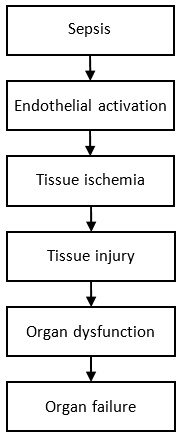
\includegraphics[width=0.2\textwidth]{figures/SepsisEndo}
	\caption{Scheme that shows the progression from sepsis to organ failure. Modified from S.Baudouin.\cite{baudouin2008}}
	\label{fig:Sepsis}
\end{figure}

Summarized, sepsis affects the processes within the microcirculation to an extent that the impairment exceed the autoregulation abilities of vasomotion.
%Infrared Thermography 
\chapter{Infrared Thermal Imaging}

This is imaging of thermals 


Thermal imaging is an technique that utilizes infrared radiation emitted from nearly any objects. 
The existence of infrared radiation was first discovered in 1800 by Sir Frederick William Herschel. 
His experiments lead to the knowledge that there were a light spectrum beyond the visual spectrum humans are able to perceive.\cite{ignacio2017,optris2009}

Thermal imaging is commonly used to calculate surface temperatures. Two important concepts, heat and temperature emerge in the understanding of this. Temperature is a measure for the internal energy within an object and can be defined as the average kinetic energy of the object.
Heat is the energy that passes from a warm object to a colder object. Warm objects will decrease in internal energy and cold objects will increase due to the temperature difference and therefore the heat transfer. In the human body, a constant temperature is keep, due to several factors and therefore the temperature will not decrease even though a heat transfer to the surrounding environment occurs. The environmental temperature do have an impact on how large the heat transfer gradient is. If a body is in a cold environment, the emitted heat will be greater than the absorbed. In the same way, if the environment is much warmer than 37$^{\circ}$C, a greater absorption than emission will occur and the body will increase in temperature.\cite{ignacio2017} 

\section{Measuring thermal energy}

The theory of the black body is important to understand the absorption and emission of light relative to temperature. Because the theory of the black body is used to describe the laws of infrared radiation and its relationship to temperature. The black body is an ideal perfect emitter of infrared radiation because it absorbs all electromagnetic radiation permitted to it, and it emits the same amount of radiation as it absorbs, the absorption and emission are both equal to one. 
Spectral emissive power, also denoted $E_\lambda$ is the energy emitted by a surface in relation to time and range of wavelength. Figure \ref{fig:Spectral} shows an graphical illustration of spectral emissive power of the black body for specific wavelengths when the temperature changes. \cite{ignacio2017} 

\begin{figure}[H]
	\centering	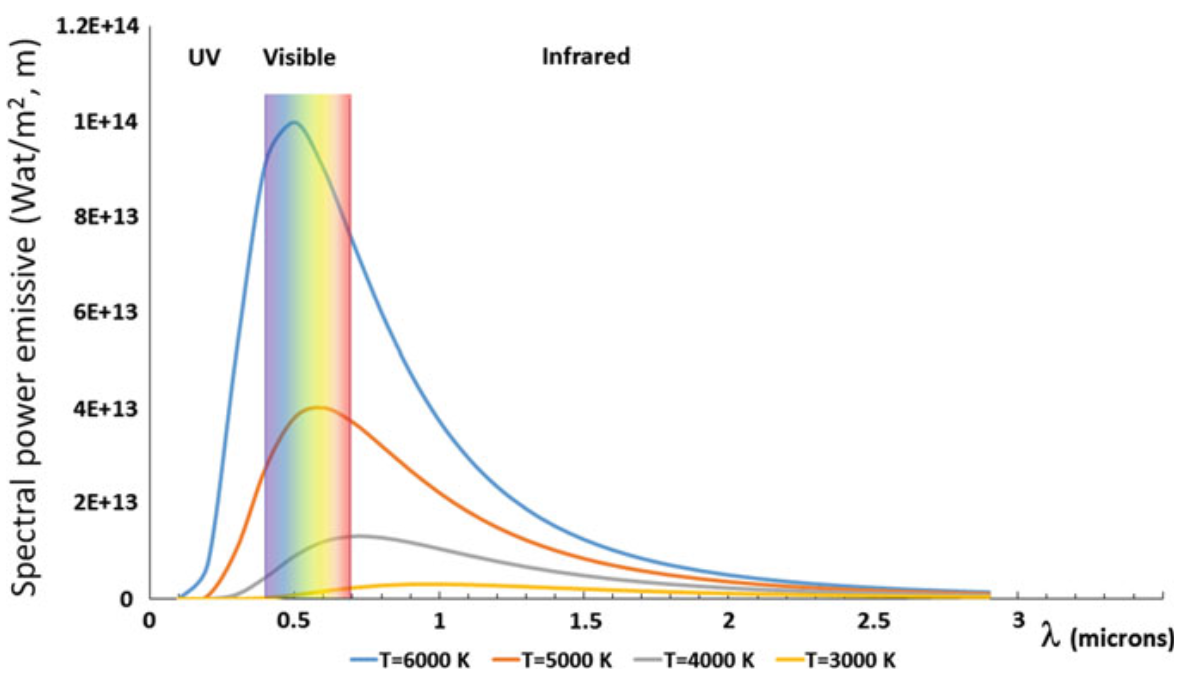
\includegraphics[width=0.65\textwidth]{figures/Spectral_power_emissive}
	\caption{Spectral power emissive as a function of wavelength for different temperatures \cite{ignacio2017}}.
	\label{fig:Spectral}
\end{figure} \vspace{-.3cm}

The knowledge of this principle helps in the understanding of how infrared radiation behaves, and how temperature affects the wavelength of the signal. 
The radiation from the human body which has a temperature at 37$^{\circ}$C emits the maximum energy of $9.3 \mu$m, which means that most of the radiation is in the far infrared spectrum.\cite{ignacio2017}

Physical laws including Wien's displacement law and Stefan-Boltzmann's law are important for explaining how the infrared radiation behaves at different temperatures. \cite{ignacio2017} 

Wien's displacement law explains that the wavelength of the peak of the black body radiation curve decreases as the body temperature increases. This law can be used to describe different wavelengths according to the temperature of the black body which emits the radiation. Wien's law has the following equation: 

\begin{flalign}
	\lambda_{max} = \frac{a}{T}
	\label{eq:wien}
\end{flalign}

$a$ has a value of $2.897*10^{-3} m K$ and denotes the Wien's displacement constant. $T$ denotes the absolute temperature in kelvin. $\lambda_{max}$ denotes the wavelength of emission peak with unit in meters.\cite{ignacio2017} 

Stefan-Boltzmann's law explains that small changes in temperature will lead to big changes in emissive power. This is seen in Stefan-Boltzmann's equation because it states that the total emissive power is proportional to the fourth power of the absolute  temperature. \cite{ignacio2017}

\begin{flalign}
	E = {\varepsilon}*{\sigma}*{T^4}
	\label{eq:stefan}
\end{flalign}

In Stefan-Boltzmann's equation $E$ denotes the total emissive power with unit $W/m^{2}$. $\sigma$ denotes the Stefan-Boltzmann's constant, and has a value of $5.67*10^{-8} W/m^{-2} K^{-4}$. $T$ is the temperature in kelvin. $\varepsilon$ denotes the emissivity and is normally not a part of the Stefan-Boltzmann's law, but part of the modified Stefan-Boltzmann's equation, because it is used for calculation of temperature in most thermal cameras. 

Emissivity is different for all materials. Skin have an emissivity between 0.95 to 9.99, why these values typically are used when assessing the temperature of the skin of the human body with thermal imaging.
This law is important when considering thermal imaging because the sensitivity when calculating the temperature from the emissive power is considerable. \cite{ignacio2017}

\textbf{Region of interest}

Region of interest (RIO) is an important consideration when doing measurements with thermal imaging. One of the reasons why this is an important aspect is because it is the RIO that lays the foundation of the data that goes into the statistical analysis. A minimum of 25 pixels is recommended for the RIO to reduce error in the data. To get the best measurement the RIO should be filling most of the image to get the best thermal data and better resolution in the area you want to measure.\cite{ignacio2017}  \fxnote{This is very badly explained. It it needed?} 

\textbf{Thermal cameras} \label{sec:cam}

The radiation emitted from an object is focusing the RIO onto an array of detectors via a lens in the thermal camera. The array is also called the focal plane array and consists of typically $384 * 288$ to $1024 * 768$ single microbolometers.\cite{olbrycht2015} The radiation emitted to the detectors generates an electric output proportional to the radiation. The output is then undergoing amplification before further signal processing that digitalizes the signal into pixels. This allows the final output signal to be viewed as a temperature for the object on an monitor, this is also illustrated on figure \ref{fig:em_spectrum}. \cite{optris2009}

\begin{figure}[H]                                         
	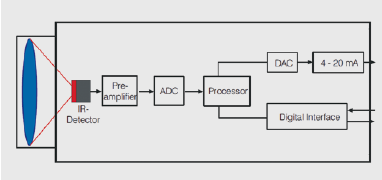
\includegraphics[width=.55\textwidth]{figures/IR_cam}  
	\caption{Simplified block diagram of an standard infrared camera.\cite{optris2009}}
	\label{fig:em_spectrum}  
\end{figure} 

The infrared radiation is made into an electrical signal in the camera, this data can be used in calculating the temperature for an object by knowing certain variables and putting these into Stefan Boltzmann's equation \ref{eq:stefan}. The emissive power denoted E, is the radiation that the detector in the camera is getting. The variables $\sigma$ are known and $\varepsilon$ is specified for the object that is being measured, eg. the human skin with emissivity between 0.95 to 0.99. The temperature are then the only variable to calculate and this is done for each pixel in the image to make up the complete thermal image of the object. Each pixel will be representing one thermal data. \cite{ignacio2017}


%\section{Physical principals}
%
%Any object above absolute zero emits energy-electromagnetic radiation depending on its temperature. Absolute zero is $0K$ or $ -273.16^{\circ}$C. To put that into perspective the human body has a temperature around 37$^{\circ}$C.\cite{ignacio2017,optris2009}
%
%Electromagnetic radiation is a propagation of energy trough a medium without the transportation of mass. An electromagnetic wave is made of the relationship between frequency $f$, wavelength $\lambda$ and the speed of light $c$. This is stated in the equation of wave motion.\cite{ignacio2017}  
%\begin{flalign}
%	\lambda = \frac{c}{f}
%	\label{eq:wave}
%\end{flalign}
%Depending on the frequency and wavelength certain characteristics arise from what is called the electromagnetic spectrum. The electromagnetic spectrum is the electromagnetic energy that is emitted. This extends from radiation of low energy such as radio waves and infrared, to waves of higher energy in form of eg. X-rays. A graphical representation of the electromagnetic spectrum can be seen on \cref{fig:em_spectrum}.\cite{ignacio2017}        
%
%\begin{figure}[H]                                         
%	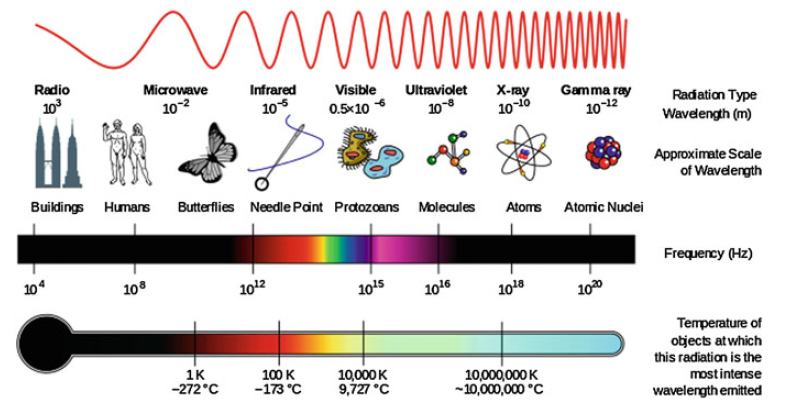
\includegraphics[width=.66\textwidth]{figures/em_spectrum}  
%	\caption{The electromagnetic spectrum with wavelength, emitters, frequency and temperature.\cite{ignacio2017}}
%	\label{fig:em_spectrum}  
%\end{figure}   
%
%Infrared radiation is also known as thermal radiation because of the relationship between temperature and infrared radiation. Temperature of the human body permits radiation in the infrared spectrum, but objects of much higher temperature are capable of emitting radiation in the visible and UV spectrum. This has to do with the difference between object and environmental temperature. If the temperature of these are relatively close to each other, the radiation emitted will be within infrared wavelengths. Infrared radiation has a wavelength from 769 nm to 1 mm. Objects emit more radiation in some region regions compared to others. Because of this is the infrared spectrum classified in the three regions, near, middle and far infrared. Near is between 769 nm and 2.5 $\mu$m, middle 2.5 $\mu$m to 50 $\mu$m and far 50 $\mu$m to 1 mm. The human body emits most radiation in the far infrared part, and most thermal cameras are build with this in mind. Near and middle cameras are used to measure gases.\cite{ignacio2017} 
%
%
%
%
%%A bit more needs to be written here i think..
%%
%%
%%Extra notes that i'we just copied that we can use later 
%%
%%The advantages of non-contact temperature measurement
%%are obvious – it supports:
%%
%%• Temperature measurements of moving or overheated
%%objects and of objects in hazardous surroundings
%%
%%• Very fast response and exposure times
%%
%%• Non-interactive measurement, no influence on
%%the measuring object
%%
%%• Non-destructive measurement
%%
%%• Measurement point durability, no mechanical wear





%Infrared and Vasomotion
\chapter{Methods of studying vasomotion}

\textit{In the following chapter an introduction to different techniques of measuring vasomotion will be given. Here methods and applicability for measuring vasomotion will be presented, with main focus directed towards thermal imaging and important parameters using this technique. }
%%\section{Techniques of measuring vasomotion} 
\label{freq}

For some time it has been the interest of researchers and health care clinicians to get a better understanding of the mechanisms that control and regulate local blood flow in the microcirculatory system\cite{sagaidachnyi2014,sagaidachnyi2017,geyer2004,liu2012}. 
Visualization of the vessels in skin and the way these behave can be important for assessment of stages of sepsis as mentioned before in \cref{chap:sepsis}, but also in peripheral vascular disease, the results of skin reconstructive surgery, wound and ulcer management.\cite{liu2012,kanta2014}
Spectral components of vasomotion seem to vary when influenced of some diseases. An example could be a decrease in amplitude of endothelial blood flow oscillations is assumed to be a biomaker for endothelial dysfunction. Endothelial dysfunction indicate cardiovascular disorders such as arterial hypertension and cardiac ischemia. An increased amplitude within the neurogenic frequency band is characterized by a decrease of vascular resistance and an increase of blood flow through the arteriovenous shunt.\cite{sagaidachnyi2017}

For measuring regulation in the peripheral blood flow, it is assumed that these oscillating changes are the source of thermal waves propagating from microvessels toward the skin surface. Especially thermal imaging uses this concept.\cite{sagaidachnyi2017}
Furthermore a correlation between skin temperature in fingertips and blood flow oscillations has been found\cite{sagaidachnyi2014}.
When the thermal waves propagate from the vessels towards the skin surface they are prone to some attenuation. This is due to skin properties that function like a low-frequency filter.\cite{podtaev2008}
The magnitude of attenuation is directly proportional to the frequency.
Therefore as illustrated in \cref{fig:atten}, a higher frequency leads to a higher attenuation.   

\begin{figure}[H]
	\centering	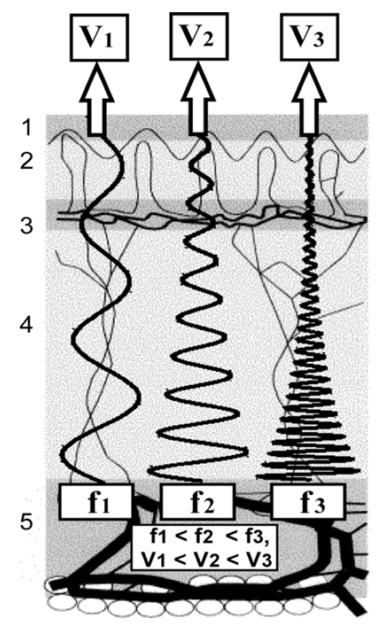
\includegraphics[width=0.28\textwidth]{figures/attenuation}
	\caption{Graphical representation of amplitude dampening in three signals with different frequency.\cite{sagaidachnyi2014}}
	\label{fig:atten}
\end{figure} \vspace{-.3cm}

There are multiple different techniques of measuring blood flow in the peripheral circulatory system. For example capillaroscopy, laser Doppler flowmetry (LDF), and thermal imaging. These have been used differently trying to quantify functional aspects of skin vasculature.\cite{liu2012} Laser Doppler flowmetry is one of the most used\cite{geyer2004} and thermal imaging being introduced as a new technique of measuring vasoregulation\cite{sagaidachnyi2014}.

\section{Thermal imaging}
\label{sec:thermalImaging}
In studies made by a Russian group by Sagaidachnyi et al. thermal imaging has been used to study vasomotion. In their studies they sought to get better understanding of the relationship between blood flow oscillations and temperature oscillations, and if it was possible to recreate the blood flow oscillation from temperature recording. Recordings of flow were done by Photoplethysmography and temperature of the skin by thermal imaging. The recordings were made on a small point of the fingertip. Trough their work, five frequency bands were identified as vasomotion activity, and are following: endothelial (0.005–0.02 Hz), neurogenic (0.02-0.05 Hz), myogenic (0.05-0.15 Hz), respiratory origin (0.15-0.4 Hz) and cardiac origin (0.4-2.0 Hz).\cite{sagaidachnyi2017,sagaidachnyi2014}
The choice of using thermal imaging to study vasomotion implies certain advantages. Mainly a larger sample area, but also a higher temporal, (up to 105 fps) and spatial (2048 × 1536 pixels) resolution. In addition it is also a non invasive way of measuring vasomotion.\cite{sagaidachnyi2017}

\section{Laser Doppler flowmetry}
In an other study from Geyer et al. vasomotion is investigated trough the use of laser Doppler flowmetry as recording technique. In the study vasoregulation variables are sought quantified. LDF is a non invasive approach to measuring changes in vasomotion. The technique register changes in the depth of 1 mm, and works like Doppler ultrasound, utilizing the shift in frequency. Though instead of using ultrasonic waves, LDF uses light reflected from red blood cells. This study found the same frequency bands as Sagaidachnyi et al. with minimal difference. Data obtained were analyzed trough spectral analysis. Wavelet transform was used instead of the most used fourier analysis, because wavelet analysis offered better resolution to reveal characteristics in the low frequency area.\cite{geyer2004}
LDF uses a small sample area and the laser probe allows a sampling area as small as 1 mm$^3$.\cite{brothers2010} 


  
\section{Summarizing}

Both Geyer et al. and Sagaidachnyi et al. managed to show spectral components relating to vasomotion. The techniques both uses an non invasive approach, even though the methods are different when measuring red blood cell count compared to temperature. The use of thermal imaging as the method of measuring vasomotion offers interesting opportunities. Larger sampling area would allow interpretation and study of a more global tissue area. Along with the resolution of thermal imaging cameras, this makes thermal imaging the choice of measuring technique to be used in this study. 




%Method
\chapter{paired t-test}

The used method of the study design is called in series design. This enable to compare the situation before and after treatment within each subject.
\begin{figure}[H]
	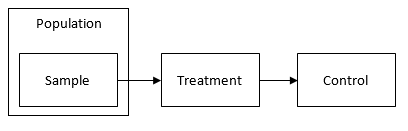
\includegraphics[width=0.4\textwidth]{figures/inseries1}
	\caption{The procedure of studies with in series design.}
	\label{fig:FigureLABEL}
\end{figure}

Within this study the arms of the subjects will be cuffed. To avoid any carry-over effect, the measurements on the normal arm will be done first. That means beginning with the control and then the "treatment".
\begin{figure}[H]
	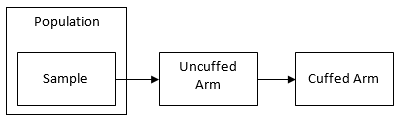
\includegraphics[width=0.4\textwidth]{figures/inseries2}
	\caption{The procedure of this study with in series design.}
	\label{fig:FigureLABEL}
\end{figure}

The paired t-test is used to check the difference of means of two conditional samples. This test is usually used to compare "before treatment" and "after treatment".
It is requisite that the sample size of the of both samples is identical.
Following some useful formulas:
\begin{itemize}
	\item test variable
	\begin{flalign}
		t=\frac{\bar{X_{D}}-\mu_{0}}{\frac{s_{D}}{\sqrt{n}}}
	\end{flalign}
	\item mean of difference of the paired means
	\begin{flalign}
		\bar{X_{D}}=\frac{1}{n}\times \Sigma (X_{1}-X_{2})
	\end{flalign}
	\item standard derivation of the difference of the paired means
	\begin{flalign}
		s_{D}=\sqrt{\frac{\Sigma((X_{1}-X_{2})-\bar{X_{D}})^{2}}{n-1}}
	\end{flalign}
	\item degree of freedom
	\begin{flalign}
		2\times n-2
	\end{flalign}
\end{itemize}
\section{Subjects}

Eight healthy subjects within the age of .. - 52 where taking part in the experiment as volunteers, three men and one female. The research is done as a pilot study, why it is presumed that the sample size of eight is sufficient. The research focuses on assessing the microvasular system with the hand as a window on healthy subjects, why the following inclusion and exclusion criteria have been formed:

\textbf{Inclusion criteria}
\begin{itemize}[noitemsep]
	\item Subjects should have at least one hand to perform the measure on
	\item The cuff should be able to fit the arm circumference 
	\item The subject should be able to sit still for a greater extend of time
\end{itemize}

\textbf{Eksclusion criteria}
\begin{itemize}[noitemsep]
	\item Health conditions that sets the subject in risk of injury when conducting the experiment like high blood pressure.
	\begin{itemize}
		\item Systolic blood pressure over 140
		\item Diastolic blood pressure over 90
	\end{itemize}	
	\item Age under - years old
	\item Age over - years old
	\item Obesity to a greater extend
	\item Parkinson disease  
\end{itemize} 

The experiment was performed in a small laboratory office at Hjørring hospital in of Northern Denmark. 
\section{Test setting}

The subject was placed in a upholstered chair with adjustable backrest, footrest and armrests, which allowed a good positioning of the measured hand, while the subject remained in a relaxed position. Measurements were carried out on the dominant hand. The hand was stabilized with a vacuum pillow which was covered by a micro fiber tissue to get a better background for the images. Microfiber has a low heat conduction \cite{schacher2000}. That helps to identify the outlines of the hand on the thermal image, because the tissue is not conducting the temperature of the hand to a high extent. To provide a more comfortable position of the arm during the experiment the armrest of the adjustable chair was padded with some sheets under the vacuum pillow. A comfortable position in the chair was important, because the subject had to sit still and was not allowed to move during the test for at least 45 minutes These precautions only counteracted some small movement, and therefore it was important that the subject was focused on sitting still. 
$37.5\pm 1$ cm over the hand the Gobi $640$ $17\mu$m GigE, sensitivity 0.005$^\circ$, resolution 480 x 640 infrared camera (Xenics NV, Belgium) was positioned with a tripod. The setup with camera, chair and computer can be seen on \figref{fig:setting}. 


\begin{figure}[H]
	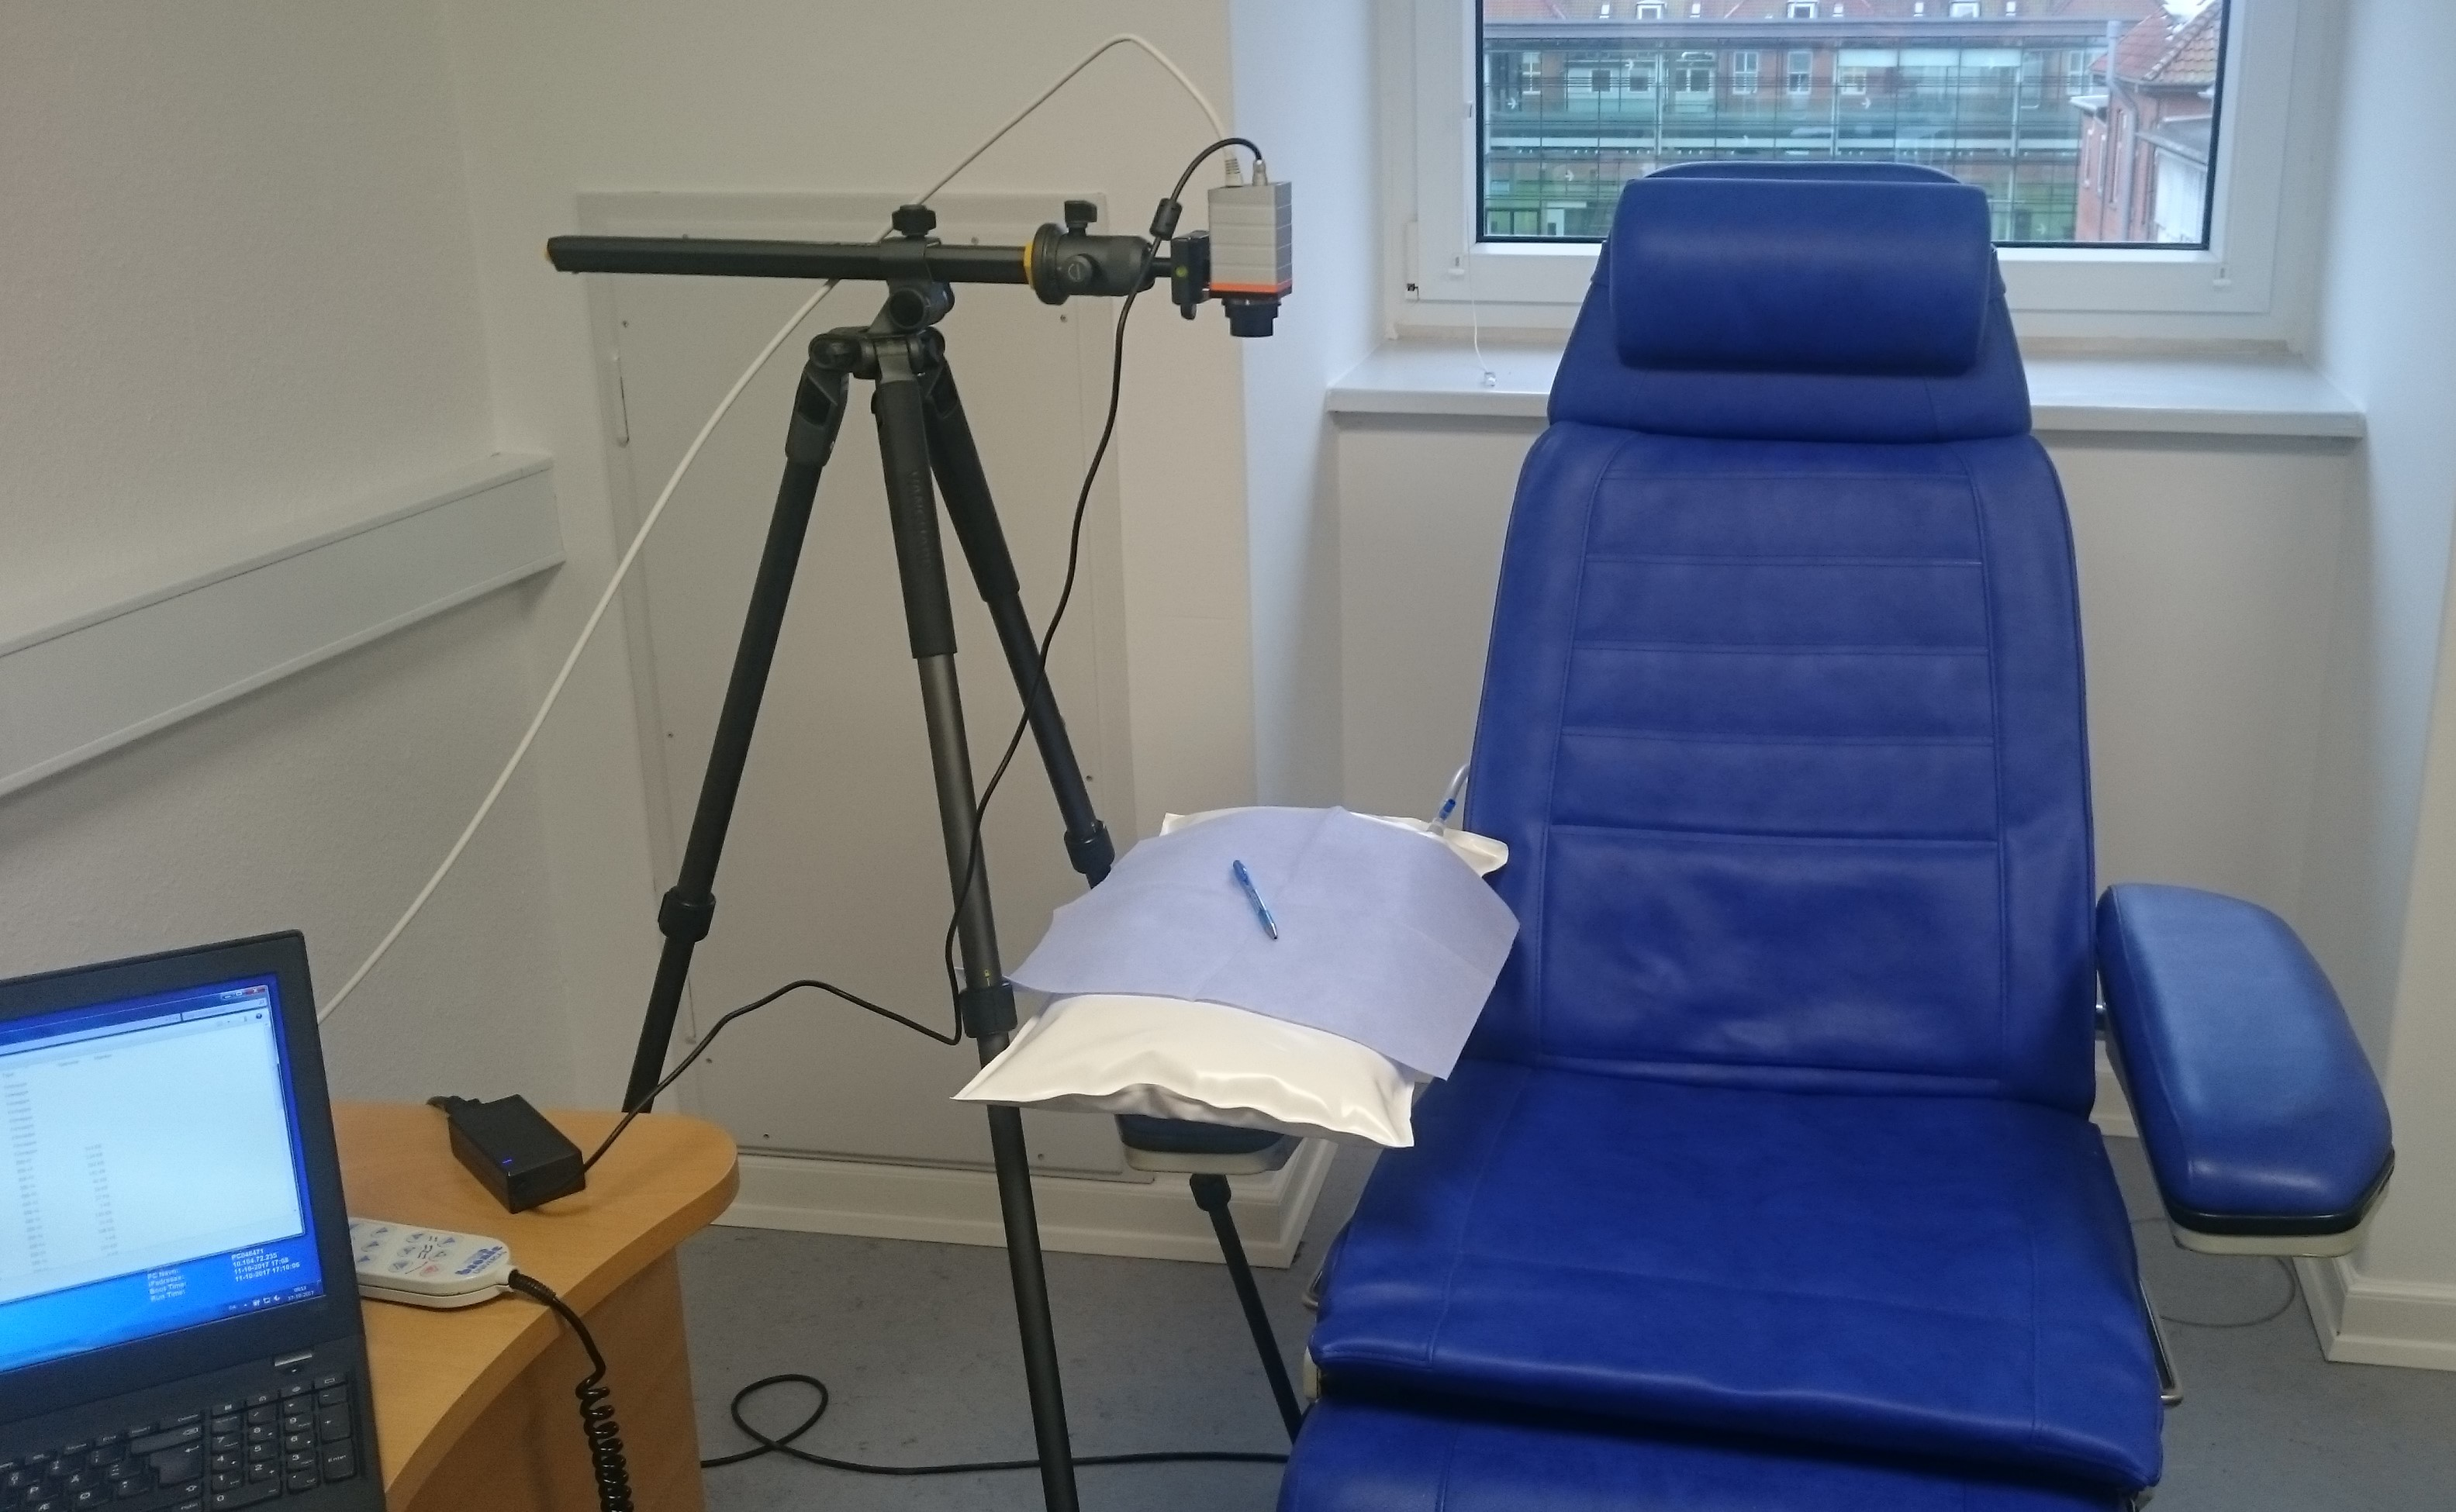
\includegraphics[width=0.7\textwidth]{figures/setting}
	\caption{The test setting at the Regionshospital Nordjylland.}
	\label{fig:setting}
\end{figure}

The camera was via a Ethernet cable connected with a laptop, which was used to record the measurements with Xeneth 2.6 software. 
First cable connections between the camera, the laptop and the power supply were set. Afterwards the camera was turned on and had to warm up for about 15 minutes. During this the laptop was started and the software for taking the measurements was set in operational readiness.

When the preparation of the test setting was done, the preparation for the subject begun. At first the blood pressure of the subject was measured on the dominant arm. The blood pressure was measured three times while the subject was sitting relaxed on a chair. Mean systolic blood pressures was calculated. To get the total occlusion pressure $(TOP)$ the mean was multiplied by 1.3. To reduce the blood flow in the arm to 50\% during the measurement within the second condition, the arm was cuffed with 30\% of the $TOP$.\cite{mouser2017} 
Then the cuff was affixed at the subjects dominant arm without tighten it, so that it was ready for the second part of the experiment. After that the subject took place in the chair and the hand was stabled with the vacuum pillow. The vacuum generator was attached to the pillow for giving the hand more stability. The lens focus has been adjusted so the distance was taken into consideration, to make sure the image was sharp.

When the camera was stable and the filename was modified according to the subject, the first measurement was started for 20 minutes. During the whole experiment the subject was not allowed to move or speak to minimize movement bias.
Directly after the first measurement the cuff on the arm of the subject was tightened with the calculated value. The pressure of the cuff had to be observed during the whole measurement and if necessary adjusted.

To guide the conductors of the experiment, an experimental protocol was formed and followed during the experiment. The experimental protocol can be seen in \cref{chap:protocol}. 



\urlstyle{same}
\printbibliography
\cleardoublepage

% BILAG
\begin{appendices}

\end{appendices}


\end{document}
